\documentclass[output=paper]{LSP/langsci} 
\ChapterDOI{10.5281/zenodo.1090970}
\title{What does a translator do when not writing?}
\subtitle{Being less naïve about indicators of cognitive effort in translation}
\rohead{\thechapter\hspace{0.5em}What does a translator do when not writing?}

\author{Daniel Couto-Vale}
\affiliation{RWTH-Aachen University}
%\\\email{danielvale@icloud.com}
\abstract{In this paper, I revisit the notion of translation unit in both a production and a product sense. In particular, I present evidence that the relation between writing bursts (production segments) and grammatical structures (product segments) is not as simple as currently assumed and that the length of writing pauses does not directly correspond to cognitive effort in translation. Finally, I contrast my approach to pauses with \citeauthor{Dragsted:2005vl}'s (\citeyear{Dragsted:2005vl}) and present evidence that typing pauses might be less biased indicators of cognitive effort than the standard writing pauses currently being used.}


\begin{document}
\maketitle


\section{Introduction}
\label{couto:sec:intro}

In process-oriented translation studies, researchers report using a diverse set of devices for tracking translator's behaviour, amongst which keystroke loggers play a central role. When observing and describing the \isi{translation process}, ``typing'' \isi{pauses} are often used as indicators of \isi{cognitive effort} \citep{Hansen:1999wn,Hansen:2002wu,Alves:2003va,PACTE:2005vu,Dragsted:2004tj,Dragsted:2005vl}. However, in most studies if not all, very little attention is given to what physically happens when someone interacts with a keyboard. In this paper, I shall explain how the keyboard layout and the translator's typing habits can enlarge and shorten the interval between two writing actions independently of how difficult the translation task is and I shall demonstrate how the writing system and the lexicogrammatical system of the \isi{target language} cause \isi{pauses} in writing of their own, which are unrelated to the translation task. Finally, I shall propose an experimental setup and a post-processing of keyboard logs aimed at discounting the time spent with translation-unrelated behaviour to achieve a better approximation of the time spent translating, that is, the time spent on intellectual bilingual activity.

\subsection{Key-moving, typing and writing actions}
\label{couto:sec:KeyMovingTypingWriting}

When a translator types, the translator moves keys down and up. These key-moving actions are called by some \textbf{key down} and \textbf{key up} (e.g. Javascript key listeners), by others \textbf{key press} and \textbf{key release} (e.g. Java key listeners), and by others \textbf{key press} and \textbf{key break}. I shall refer to them as \textbf{key down} and \textbf{key up} actions because that term pair seems the least prone to misunderstanding.

To ground this discussion, I shall start by pointing out that a keyboard is not a tool simply for inserting, replacing and removing characters in the text area. There are at least two software levels above a key-moving action\footnote{A.k.a. a keyboard event in informatics}: the typing system\footnote{A.k.a. a layout controller in informatics} and the writing system\footnote{A.k.a. an input system in informatics}.

Descriptively speaking\footnote{The description I shall make does not necessarily correspond to any actual software implementation. It is a description of typewriting for the purpose of advancing translation studies and not a documentation of any particular driver, operating system or word processor.}, a keyboard layout maps each key to a key value. Counting from left to right in rows and top down in a single column, keys may be numbered \#1, \#2, \#3... until the last key in the lower right corner of the keyboard. Keyboards vary greatly in how many keys they have. After numbering them in such a way, a keyboard layout can be understood as the mapping of a key index such as \#1, \#2, and \#3 to a unicode character such as LATIN SMALL LETTER A (U+0061), CIRCUMFLEX ACCENT (U+005E), and SPACE (U+0020).

\largerpage
Let us consider that a particular typing system has one or more of such keyboard layouts. And let us consider that some key-down and key-up actions trigger the replacement of a layout by another. For instance, let us say that Layout \emph{LC} maps the key \#60 to the value LATIN SMALL LETTER A (U+0061) whereas Layout \emph{UC} maps the key \#60 to the value LATIN CAPITAL LETTER A (U+0041). Finally, let us assume that both layouts map the key \#87 to the value SHIFT IN (U+000F). Now let’s say that there is a layout controller that does the following. It keeps a \textbf{U+000F key state}, which can be either \textbf{low} or \textbf{high} and it updates the shift key state to low whenever the \textbf{U+000F key down action} is performed and it updates that state to high whenever a \textbf{U+000F key up action} is performed. Moreover, let us assume the layout controller applies Layout \emph{LC} to key-moving actions whenever the shift key state is high and applies Layout \emph{UC} to them whenever the shift key state is low.

\newpage 
Finally, let’s suppose a writing system works in the following way. The writing system would have a typing layout that maps typing actions to writing actions. For instance, a particular typing layout would map the typing action \textbf{U+0061 key down} to the writing action \textbf{U+0061 char insert}, the typing action \textbf{U+0041 key down} to the writing action \textbf{U+0041 char insert}, while assigning the typing actions \textbf{U+0041 key up}, \textbf{U+0041 key up}, \textbf{U+000F key down}, \textbf{U+000F key up} to no writing action.

Assuming the above process, the following key-moving actions would be recognised as the following typing actions, which in turn would be recognised as the following writing actions (see \tabref{couto:tab:1}). The fourth column contains the resulting text with the resulting cursor position (see \sectref{couto:sec:TextVersions} for more on text versions and cursor positions).

\begin{table}%1
\begin{tabular}{llll}
\lsptoprule
key-moving & typing & writing & resulting text \\
\midrule
\#60 key down & U+0061 key down & U+0061 char insert & a| \\
\hline
\#60 key up & U+0061 key up & & a| \\
\#87 key down & U+000F key down & & a| \\
\#60 key down & U+0041 key down & U+0041 char insert & aA| \\
\hline
\#60 key up & U+0041 key up & & aA| \\
\#87 key up & U+000F key up & & aA| \\
\#60 key down & U+0061 key down & U+0061 char insert & aAa| \\
\hline
\#60 key up & U+0061 key up & & aAa| \\
\#60 key down & U+0061 key down & U+0061 char insert & aAaa| \\
\hline
\#60 key up & U+0061 key up & & aAaa| \\
\lspbottomrule
\end{tabular}
\caption{Key-moving, typing, and writing actions}
\label{couto:tab:1}
\end{table}

Here is where the first issue lies. A large portion of \isi{translation process} studies was developed with ``key-logging'' software that does not record key-moving and typing actions. One of the most used software in translation studies is Translog® and it only records writing actions. However, as we can see in \tabref{couto:tab:1}, inserting some characters such as `A' (U+0041) takes more typing actions than inserting other characters such as `a' (U+0061): the first char insert action is realised by moving down the shift key to switch the keyboard layout and by moving down the U+0041 key (both keys need to be moved up afterwards); the second char insert actions is realised simply by moving down the U+0041 key. Because of this, the interval between inserting the char `a' and the char `A' is likely to be larger than the interval between the char `a' and the char `a'. Similarly, because the number of keys that need to be moved up after inserting the char `A' is larger than after inserting the char `a', the interval between inserting the char `A' and the char `a' is likely to be larger than the interval between the char `a' and the char `a'.

In this way, if we take the whole time between two char insertions to be a pause in typing/writing, two typing/writing \isi{pauses} of the same length may include sequences of finger movements of various lengths. If we do this, we can make no claim that similarly long \isi{pauses} correspond to a similar amount of \isi{cognitive effort} since part of this time is spent moving keys down and up after a decision of what to write has been made.

The ideal and long-lasting solution for this issue would be to update `key-logging' software so as to start logging key-moving and typing actions. With this new kind of log, we would be able to see when typing indeed stops and when it indeed resumes. However, in the absence of a more precise solution and in the presence of large expensive corpora containing solely writing actions, I shall propose a way to treat writing \isi{pauses} in a less naïve way so that some correspondence between such \isi{pauses} with typing-unrelated effort can be established (see \sectref{couto:sec:HandlingPauses}).

\subsection{Text Versions}
\label{couto:sec:TextVersions}

Let us assume, as some linguists do \citep{Hasan:1999um}, that a human language `includes' texts.\footnote{This section does not focus on the dichotomy between \isi{text production} and text as product.}\textsuperscript{,}\footnote{The notion of series of text versions, which applies both to translation and to other kinds of \isi{text production}, is not covered by \citeauthor{Vermeer:2004tw}'s model of translation.}\textsuperscript{,}\footnote{The understanding of a final target text as a translation product (``translatum'') as proposed by \citeauthor{Vermeer:2004tw} in his Skopos Theory (\citeauthor{Vermeer:2004tw}, \citeyear{Vermeer:2004tw}[1989]) follows the ancient dichotomy between \isi{text production} (\textit{ἡ ποίησις} `poiesis') and text as product (\textit{τὸ ποίημα} `poiema'), which traces back to Plato's discussion about who the narrator of Iliad and Odyssey is. Similarly to the difference in function (``Skopos'') between an original text and its translations, ancient rhetoricians were concerned with the fact that Homer composed Iliad and Odyssey once whereas several citar-playing singers performed those epoi multiple times throughout the ages.} That means, when a text is received, it not only occurs but also becomes an option of what to say in a language. Let us also assume that a language is the meaning potential in Halliday's sense, in other words, that it is not a lexical or grammatical potential in \citeauthor{Chomsky:1957bv}'s sense\footnote{According to \citeauthor{Chomsky:1957bv}, a language consists of all words and all grammatical rules for combining them.} (\citeyear{Chomsky:1957bv}) and that it is not a graphological potential in \citeauthor{Eddington:1929vg}'s sense\footnote{This tradition of making arguments by supposing a random choice of letters traces back to Cicero when he stated that the annals of Ennius could be written by throwing a bag of metal letters on the floor whereas a poetry verse could not be created in such a careless way (D\={e} n\={a}t\={u}r\={a} de\={o}rum II, 37 § 93).}\textsuperscript{,}\footnote{During the development of set and probability theory, \citet[p. 194]{Borel:1913vy} conceived of texts again as strings, i.e. as sequences of characters. According to him, a team of illiterate typists would create random sequences of characters and would create one day by chance all texts conserved in the largest national archives. Eddington made the same argument for monkeys typing the texts in the British Museum.} (\citeyear{Eddington:1929vg}, p. 72). From such a perspective, a physical text is a print of a semantic form, which also gets called `text'. For that reason, two distinct prints of `the same play' can be understood as being `two physical texts' \emph{as instances} (token) but also as expressing `the same text' \emph{as a semantic form} (type). In that linguistic sense, each text version during translation is a separate text (\emph{a separate instance}) and each new text version that is different from all previous ones expresses a new text (\emph{a new semantic form}). In other words, from this perspective, language is a semantic potential, not a lexicogrammatical nor a graphological potential, in the same way as a text is a semantic form, not a lexicogrammatical form (a sequence of words) nor a graphological form (a sequence of characters).


From a formal perspective, a semantic form such as the play Romeo \& Juliet is realised by a grammatical form in the sense that the semantic structure is associated with a corresponding lexicogrammatical structure (a sequence of words). In turn, the lexicogrammatical form is associated with a graphological form in so far as the lexicogrammatical structure is associated with a graphological structure (a sequence of characters). At the graphological stratum, when only one resolution, one font, one font format (size, font style, weight, colour, fill colour, underline, baseline shift, character spacing, shadow, etc.), and one single-column text area are available, a graphological form consists solely of a sequence of characters, and a graphological structure is an instance of that sequence of characters. Finally, at the graphic stratum, a graphological structure resulting from a combination of resolution, fonts, font formats, text areas and character sequences is associated with a graphic structure, which can be a series of different coloured pixels in a grid on screen or on paper (digital alternative), or a series of glyphs stamped, carved, or drawn (analogical alternative).

When studying the \isi{translation process} with the help of key-logging software such as Trans\-log®, the graphological stratum is strongly constrained. The only graphological system that a translator has control over is the one that is responsible for the selection of character sequences. It is this limited stratum (the graphological stratum) that interacts with the writing process. In this restricted environment, each character sequence is a different graphological form that is completely or partially associated with a text at the semantic stratum. And, in this context, each writing action such as \textbf{U+0041 char insert}, \textbf{left char erase}, and \textbf{right char erase} alter the graphological form and potentially the associated grammatical and semantic forms. Therefore, these writing actions are actions of replacing one text by another. In that sense, during a translation, we can talk about a series of target texts. Each pair of consecutive target texts is the input and the result of a text-replacing action, which is a writing action.

I shall follow \citet{Halliday:1987th} and call each node in this series of texts a \textbf{version}. The \textbf{initial version} is an empty character sequence, and the \textbf{non-initial versions} are the \textbf{products of writing} or simply \textbf{products}, the \textbf{final version} is the \textbf{final product [of writing]}, and \textbf{non-final products} are \textbf{intermediate versions}. Finally, \textbf{intermediate products [of writing]} are what \citeauthor{Halliday:1987th} calls \textbf{drafts}.

However, not all writing actions are meant to replace a text by another. Some of them change the state of the a text in \isi{text production}. Some typing and mouse/trackpad actions are associated with cursor motions such as \textbf{cursor back}, \textbf{cursor forward}, \textbf{cursor up}, \textbf{cursor down}, \textbf{cursor to [x]}, \textbf{cursor to line start}, \textbf{cursor to line end}, \textbf{cursor to area start}, \textbf{cursor to area end}, and with text span selection such as \textbf{back select}, \textbf{forward select}. Those are text-affecting actions that alter the state of a text (dot and mark positions) but do not replace a text by another.

In the process of writing, mouses/trackpads present an additional methodological issue for empirical studies of \isi{cognitive effort} in translation. Mouse actions associated with writing actions such as \textbf{cursor to [x]} demand the displacement of either the right or the left hand from the keyboard onto a mouse or a trackpad. However, this action is logged either only at the advent of a mouse click or from the moment the pointer starts moving. The time taken for the hand to reach the mouse/trackpad is also part of this action but is not logged. I see no solution in the short term to detect the point in time when the writing action of placing the cursor at a position with the mouse starts ,since we cannot easily track with current technology when a translator starts moving his or her hand onto the mouse/trackpad. Moreover, due to their relatively infrequent occurrence, an estimation of the duration of mouse/trackpad-related non-tracked hand-motion shall not be attempted in this paper.

\subsection{Pauses in Typing}
\label{couto:sec:PausesInTyping}

% TODO I bring evidence for the thesis that unit boundary is not what motivates \isi{pauses} and that \isi{pauses} are not evidence of unit boundaries. Instead, process unit boundaries, source unit boundaries and target unit boundaries are evidence of how the \isi{translation process} works. "I think here you talk about "the meaning of \isi{pauses}" rather than just the \isi{pauses}."

Still in the process of writing, there is another much more frequent and yet non-tracked hand-motion: simple typing. Typing has been often described as happening in bursts. In that description, typing would be cuttable into units of text-production separated by typing \isi{pauses}. In that sense, typing rhythm would be a good behavioural evidence for underlying cyclic cognitive processes. However, even though a cyclic \isi{translation process} is a reasonable model of what happens during translation, the analysis of typing rhythm has not been an unbiased one. Researchers did not start studying typing rhythm without an expectation of what they would find. They were in a search for evidence that a particular model of translation was the case. In other words, a cyclic cognitive model was assumed and evidentiated with typing rhythm.

The assumed translation cycle consists of three steps: 1) a character sequence associated with a complete grammatical structure of the source text is read, 2) then the source text segment is mentally translated into a target text segment (semantic structure), and 3) only then a character sequence realising an equivalent grammatical structure would be fully written. Given the underlying model of translation, it became imperative that the typing bursts and consequent writing bursts resulted in additions of grammatical units.

This naïve assumption that translation cycles would be the sole reason for typing bursts is pervasive and is at the core of descriptions of \isi{translation process}. These studies aim at relating spans of writing actions (typically between \isi{pauses} of a given size) with a \textbf{grammatical structure under translation}. However, this naïve assumption of direct correspondence between typing bursts and a translation cycle opposes on the other extreme a rather counter-intuitive assumption that random or non-grammatical segments of the character sequence of the source text are read and translated at a time.

Because the counter assumption is so unlikely to be the case, I do not want to give the impression that this cyclic process is not a reasonable approximation of what happens, but I shall claim that the boundaries of the source text segment under translation is by no means the only reason why a \isi{typing pause} occurs between the production of two adjacent grammatical structures. As I shall point out next, there are several other reasons for a pause to occur that are completely unrelated to a `grammatical structure under translation'. I shall bring some examples of places where I found translation-unrelated typing \isi{pauses} in writing for supporting this viewpoint. Examples are in \ili{German}. They are sequences of \textbf{char insert} actions separated by either breve (\u{ }) or long (\={ }) typing \isi{pauses} (see \sectref{couto:sec:HandlingPauses} for an explanation of these pause lengths in terms of milliseconds and for estimations of \isi{typing pause} length based on writing pause length). The symbol $\cdot$ indicates a \textbf{space char insert} action.

\begin{exe}%1
  \ex\label{couto:ex:1}$\cdot$\u{ }A\u{ }u\u{ }f\u{ }w\u{ }a\u{ }n\u{ }d\={ }s\u{ }$\cdot$ (Translator 2)
\end{exe}

\begin{exe}%2
  \ex\label{couto:ex:2}$\cdot$\={ }F\u{ }ä\u{ }h\u{ }i\u{ }g\={ }k\u{ }e\u{ }i\u{ }t\u{ }$\cdot$ (Translator 2)
\end{exe}

\begin{exe}%3
  \ex\label{couto:ex:3}$\cdot$\={ }7\={ }5\={ }$\cdot$ (Translator 2)
\end{exe}


In Example \ref{couto:ex:1}, the pause we see happened between two bound morphemes of a genitive noun in \ili{German}. In \ili{German}, there are two alternative character sequences that can realise the suffix for this genitive word, namely \emph{\uline{es}} as in \emph{Aufwand\uline{es}} or \emph{\uline{s}} as in \emph{Aufwand\uline{s}}\footnote{Explaining how the standard (phylos) of human language named Modern High \ili{German} developed from other standards in the past (phyloi) demands an observation timeframe of hundreds of years (phylogenetic timeframe). Since the current observation timeframe is of a few seconds (logogenetic timeframe), etymological considerations such as the appearance of such suffixes should play no role.}. Both character sequences realise the same grammatical structure, one being possibly more expected than the other in the situation type that the text implied. However, this grammatical structure -- a bound morpheme -- does not correspond to any bound morpheme in the English source text. Therefore, the pause does not correspond to the boundary of a grammatical structure under translation. \tabref{couto:tab:2} shows a reconstruction of the typing process based on the writing actions we have in our logs. The longer pause between \textbf{U+0064 char insert} and \textbf{U+0073 char insert} is represented by a table break.

\begin{table}%2
\begin{tabular}{llll}
\lsptoprule
key-moving & typing & writing & resulting text \\
\midrule
\#87 key down & U+000F key down & & | \\
\#60 key down & U+0041 key down & U+0041 char insert & A| \\
\#60 key up & U+0041 key up & & A| \\
\#87 key up & U+000F key up & & A| \\
\hline
\#45 key down & U+0075 key down & U+0075 char insert & Au| \\
\#45 key up & U+0075 key up & & Au| \\
\hline
\#63 key down & U+0066 key down & U+0066 char insert & Auf| \\
\#63 key up & U+0066 key up & & Auf| \\
\hline
\#24 key down & U+0077 key down & U+0077 char insert & Aufw| \\
\#24 key up & U+0077 key up & & Aufw| \\
\hline
\#60 key down & U+0061 key down & U+0061 char insert & Aufwa| \\
\#60 key up & U+0061 key up & & Aufwa| \\
\hline
\#82 key down & U+006E key down & U+006E char insert & Aufwan| \\
\#82 key up & U+006E key up & & Aufwan| \\
\hline
\#62 key down & U+0064 key down & U+0064 char insert & Aufwand| \\
\#62 key up & U+0064 key up & & Aufwand| \\
\hline
\#61 key down & U+0073 key down & U+0073 char insert & Aufwands| \\
\#61 key up & U+0073 key up & & Aufwands| \\
\lspbottomrule
\end{tabular}
\caption{Key-moving, typing, and writing actions for Example \ref{couto:ex:1}}
\label{couto:tab:2}
\end{table}

Now, let us move to Example \ref{couto:ex:2}. Here we find a very interesting pause from a cognitive perspective. As far as lexicogrammatical composition is concerned, here we have the lexical item \emph{\uline{Fähigkeit}} as in \emph{die \uline{Fähigkeit} einer Papierkugel {[}das zu tun{]}} `the \uline{capacity} of a paper ball {[}to do that{]}'. This lexicogrammatical structure is a mention of a paper ball's capacity to do something which is lexically agnate to \emph{die \uline{Kraft} einer Papierkugel {[}das zu tun{]}} `the \uline{power} of paper ball {[}to do that{]}'. In this case, \emph{\uline{Fähigkeit}} is in the same lexical set as \emph{\uline{Kraft}}. These two lexicogrammatical structures are also grammatically agnate to other more congruent representations of the same physical phenomenon such as \emph{die Papierkugel ist \uline{fähig} {[}das zu tun{]}} `the paper ball is \uline{capable} {[}of doing that{]}', \emph{die Papierkugel \uline{kann} {[}das tun{]}} `the paper ball \uline{can} {[}do that{]}', and \emph{die Papierkugel {[}\uline{leistet} das{]}} `the paper ball {[}\uline{offers} that{]}'. Because all these representations are agnate, we can expect that translators could have considered two or more of those options when translating that passage. In particular, as an alternative to \emph{die \uline{Fähigkeit} einer Papierkugel {[}das zu tun{]} ist ein Faktum} `the \uline{capability} of a paper ball {[}to do that{]} is a fact', the same translator might have considered an alternate representation such as \emph{die Tatsache, dass eine Papierkugel \uline{fähig} ist, {[}das zu tun{]}, ist ein Faktum} `the fact that a paper ball is \uline{capable} {[}of doing that{]} is a fact'\footnote{The way other translators chose to translate this passage reveals that such a structure was considered by at least some of the translators.}. However, when comparing the lexical options of grammatically agnate translation alternates, a particular pair of lexical items shows a graphological resemblance (resemblance in terms of character sequences): in the same way as in English, the Base morpheme of the words \emph{\uline{Fähigkeit}}/\emph{\uline{Fähigkeit}en} `\uline{Capacity}'/`\uline{Capaciti}es' resembles the base of its agnate \emph{\uline{fähig}}/\emph{\uline{fähig}er}/\emph{am \uline{fähig}sten} `\uline{capable}'/`more \uline{capable}'/`most \uline{capable}'. The resemblance between these two lexical words happens both in graphological form (sequence of letters) and in semantic form (meaning), but not in grammatical affordances (the structures they can fit in). Moreover, the resemblance is present not due to a derivation process such as the one that led the Old \ili{German} term \emph{f\={a}han/f\={a}nhanan} to evolve into the lexical items \emph{\uline{fähig} sein etwas zu tun} `being \uline{capable} of doing something' and \emph{ein Tier oder jemanden \uline{fangen}} `\uline{encarcerating} an animal or someone', but due to a synchronic graphological and semantic connection between the two. In this sense, it is quite interesting that a translator stopped shortly at the end of the overlap in graphological form between the agnate lexical words: namely, at the end of \emph{Fähig}-insertion and before \emph{keit}-insertion during \emph{Fähigkeit}-insertion. Furthermore, even if the pairing of graphological and semantic forms \emph{fähig}:\emph{Fähigkeit} could be taken as evidence for a Construction Grammar explanation of how these structures came to exist in \ili{German}, it is very unlikely that this translator had \emph{capabil}:\emph{fähig} and \emph{ity}:\emph{keit} in separate source text segments under translation, that is, that this translator translated each segment -- the one before and the one after the \isi{typing pause} -- in a different translation cycle. Even if I claim this second hypothesis is unlikely, how much of such a 
\isi{typing pause} is due to the overlap of graphological structures in the \isi{target language}, and how much of it is due to a truly bilingual intellectual process, is still unresolved at the current stage of research.

\largerpage[-2]
Finally, Example \ref{couto:ex:3} shows another process that seems unrelated to translation. The \isi{pauses} before and after writing the number \emph{75} may be in fact an indicator that \emph{75} in the source \isi{text reading} \emph{seventy five} is indeed aligned with \emph{75} in the target \isi{text reading} \emph{fünfundsiebzig} `five and seventy'. What is interesting here from an alignment perspective is that there is a pause in between \textbf{7 char insert} and \textbf{5 char insert}. Since the order of digits is different in written and spoken \ili{German}, the question that one can raise is whether part of the pause before and after those actions was due to a cognitive writing procedure in which the translator cognitively writes \emph{fünf und •siebzig •fünf und siebzig} `five and •seventy •five and seventy' and only physically writes \emph{•siebzig} `•seventy' with \textbf{7 char insert} and \emph{•fünf} `•five' with \textbf{5 char insert}. This underlying cognitive writing would imply that the \isi{pauses} before \textbf{7 char insert} and after \textbf{5 char insert} are longer than the one in between, and that is indeed what happens, these \isi{pauses} being approximately $2^6$ times the length of the middle one, which is already significantly longer than average (more on quantifying \isi{pauses} in \sectref{couto:sec:HandlingPauses}). This pause pattern does not prove that the above cognitive writing happened. Understanding this pattern as caused by such a cognitive writing is simply a way of explaining translators' behaviour, which might be plausible for some and less plausible for others that have other explanations. Alternative explanations might include, for instance, lack of practice by the translator with digit key typing: consequently, translators would switch between looking at the screen and at the keyboard before inserting the first digit and after inserting the last digit of a number\footnote{Notice that the typicality of typing \isi{pauses} and the occurrence of them in other similar co-texts do not give us information about what is going on during these \isi{pauses}. We need to observe the process as a whole and characterise each pause point on its own terms with different cognitive/behavioural hypotheses. What may be the case for one translator may not be the case for another.}.

Since there are many reasons for \isi{pauses} in typing to occur, it would be naïve to hold the assumption that such \isi{pauses} mostly indicate a grammatical structure boundary that corresponds to source text segments under translation and to a translation cycle. In other words, what I aim at foregrounding is that there is an issue with the standing assumption that typing \isi{pauses} would be mostly due to an iterative segmentation of the source text into translatable units followed by a translation of each unit. A direct mapping of typing rhythm onto translation cycles is not to be achieved when a thorough and close analysis of typing behaviour is carried out.

% TODO Disclaim the \isi{pauses} are at boundaries of grammatical units more emphatically because that is what this reviewer would like to count on. Claim that the grammatical boundaries are being projected by translators (as they should be) in order to explain what is going on and that the \isi{pauses} cannot be used as evidence that there are grammatical boundaries but solely as co-indicators of something more complex. "but still they are part of the \isi{translation process} and may give some hints on the translation units or at least the production units."


\subsection{Erase actions}
\label{couto:sec:EraseActions}

In addition to the assumption of translation boundaries at \isi{pauses}, another problematic assumption is that online revisions, i.e. revisions during the \isi{drafting phase}, are related to change in the choice of semantic features. Some of these \isi{pauses} indeed seem to be semantically motivated, whereas for many others such an interpretation seems questionable. In the following examples, the symbol \uettl{ } indicates a \textbf{left char erase} action, where \textbf{left char} is the character left of the cursor.

% Key hitting issues | Motoric issues

% Typing the adjacent character
\begin{exe}%4
	\ex\label{couto:ex:4}$\cdot$\u{ }K\={ }f\=\uettl\u{ }r\u{ }a\u{ }f\u{ }t\u{ }$\cdot$ (Translator 2)
\end{exe}

% Wrong order
\begin{exe}%5
	\ex\label{couto:ex:5}$\cdot$\={ }k\u{ }e\u{ }i\u{ }e\u{ }n\={ }\uettl\u{ }s\u{ } \={ }\uettl\u{ }\uettl\u{ }\uettl\={ }n\u{ }e\u{ }s\u{ }$\cdot$ (Translator 2)
\end{exe}

% Typing issues | Layout issues

% Typing two characters
\begin{exe}%6
	\ex\label{couto:ex:6}$\cdot$\={ }b\u{ }v\={ }\uettl\={ }e\u{ }s\u{ }t\u{ }e\u{ }h\u{ }t\u{ }$\cdot$ (Translator 2)
\end{exe}

In Example \ref{couto:ex:4}, what might have happened is something along the following lines. The translator had the right hand well positioned on the keyboard and the left hand somewhat misplaced and was aware of it. When typing, the left shift key was still under the left hand and was quickly moved down, which was followed by a \textbf{`k' key down} action with the right hand in regular speed. However, after inserting the `k' character, the time taken to insert the next character, namely `f', is longer than usual. Here, the translator might have had the need to reposition his/her left hand and accidentally moved down the `f' key instead of the `r' key. In the \ili{German} keyboard used in the experiment, the `f' key is directly below the `r' key and a badly positioned left hand is a sufficient reason for a `typo'.  After inserting `f' instead of `r', there is another long pause\footnote{It is definitely the case that some online \isi{revision} are initiated by a production failure being detected in quality monitoring processes. Missed keys are an example of such cases since it is by comparing the intended text and the produced one that such mistakes (typos) are likely to be detected and fixed.}, which is followed by a \textbf{left char erase} action. Such \isi{pauses} and such an erase action do not seem to have anything to do with any bilingual process.

In Example \ref{couto:ex:5}, something else happens. The translator ends up writing the word \emph{keines}, but in the first run of char insert actions, he or she writes \emph{keien} instead of \emph{keine}. The issue here was not one of moving the wrong keys, but one of moving the right keys in the wrong order. A good point to notice here is that the \textbf{`e' key down} action is usually performed with the left hand with a \ili{German} keyboard whereas the \textbf{`n' key down} action is usually performed with the right hand. This means that this mistaken order happened when coordinating the motion of both hands. The correction procedure is quite interesting too. Only part of the problem is solved by the first attempt, resulting \emph{keies} instead of \emph{keines}, this is again noticed and the second \isi{revision} procedure leads to the version \emph{keines}.

Example \ref{couto:ex:6} is not so simple. Here the translator ends up writing \emph{besteht}, but types two letters very quickly and with the same hand. In the \ili{German} layout used, the \textbf{`v' key} and the \textbf{`b' key} are adjacent and are both right of the index finger (the finger a translator would move these keys down with). Was it that the translator was unsure which key was the `b' key and moved both down in a sequence to decide which character to keep on screen or was it that the translator just moved both keys down accidentally? I do not have an answer for such a question. But one thing is for sure, this was not a bilingual process, not even a monolingual process in the sense of choosing what to say.

Furthermore, there is another type of \isi{revision} that seems to be related to the \isi{translation process} in a rather `non-linguistic' way. Such revisions are also not graphological, nor lexical, nor grammatical, nor semantic. Examples \ref{couto:ex:7} and \ref{couto:ex:8} illustrate these. In such cases, the translator seems to copy the source text instead of writing a target text. In Example \ref{couto:ex:7}, the character sequence under translation is \emph{demands}, the target character sequence is \emph{bedarf}. Grammatically valid alternatives in \ili{German} could have been \emph{bedürfte}, \emph{benötigt}, \emph{braucht}, and \emph{bräuchte} but no word starting with \emph{d}. Example \ref{couto:ex:8} shows a similar phenomenon: the source character sequence is \emph{paper} and the target character sequence is \emph{Papier}. However, the translator writes \emph{Pape}. Is it the case that he or she just missed typing the \textbf{`i' key}, or that he or she copied the source character sequence instead of writing the target one? Again, I do not have an answer for this, but it does not seem to be a bilingual process in the typical sense of what we understand by translation.\footnote{This source text copying does not seem to be an effect of `priming' given that the translator is unlikely to accept the \isi{source language} character sequence as a valid word in the \isi{target language}. However, the notion of priming could be applied to other examples if translators choose a marked lexical item instead of a less marked one because of string similarity or shared etymological origin of the lexical items in both languages.}$^,$\footnote{As for any other online \isi{revision} preceded by a breve \isi{typing pause}, a quality-monitoring process can be inferred for such cases.}

% Task issues | Copying ?
\begin{exe}%7
	\ex\label{couto:ex:7}$\cdot$\u{ }d\u{ }\uettl\u{ }b\u{ }e\u{ }d\u{ }a\u{ }r\u{ }f\={ }$\cdot$  (Translator 2)
\end{exe}

\begin{exe}%8
	\ex\label{couto:ex:8}P\u{ }a\u{ }p\u{ }e\u{ }\uettl\={ }i\u{ }e\u{ }r\u{ }$\cdot$ (Translator 2 : 1st `Papier')
\end{exe}

% TODO Is this a different "Papier" or a different translator? Could you please report on the data in greater detail?

Other revisions such as Examples \ref{couto:ex:9} and \ref{couto:ex:10} look more linguistic. However, they are also not grammatical: the first is a replacement of a \emph{latin small letter P} by a \emph{latin capital letter P} and the second is a replacement of \emph{latin capital letter G} by a \emph{latin small letter G}. As seen before, replacements of characters are not performed necessarily with one \textbf{left char erase} action followed by one \textbf{char insert}. It may take more than two writing actions for realising the replacement of one character: in Example \ref{couto:ex:10}, a total of eight writing actions were performed for changing one letter from capital to small. Tables \ref{couto:tab:3} and \ref{couto:tab:4} show the series of resulting texts for both examples.

\begin{exe}%9
	\ex\label{couto:ex:9}$\cdot$\={ }p\={ }\uettl\u{ }P\u{ }a\u{ }p\u{ }i\u{ }e\u{ }r\u{ }$\cdot$ (Translator 11 : 6th `Papier')
\end{exe}

\begin{table}%t3
	\centering
	\begin{tabularx}{\textwidth}{XX}
		\lsptoprule
		writing & resulting text \\
\midrule
		U+0070 char insert & p| \\
		\hline
		\hline
		left char erase & | \\
		\hline
		U+0050 char insert & P| \\
		\hline
		U+0061 char insert & Pa| \\
		\hline
		U+0070 char insert & Pap| \\
		\hline
		U+0069 char insert & Papi| \\
		\hline
		U+0065 char insert & Papie| \\
		\hline
		U+0072 char insert & Papier| \\
		\lspbottomrule
	\end{tabularx}
	\caption{Writing actions of Example \ref{couto:ex:9}}
	\label{couto:tab:3}
\end{table}

\begin{exe}%10
	\ex\label{couto:ex:10}$\cdot$\u{ }G\u{ }r\u{ }o\={ }\uettl\u{ }\uettl\u{ }g\u{ }\uettl\u{ }\uettl\u{ }g\u{ }r\={ }o\u{ }ß\u{ }e\u{ }n\u{ }$\cdot$
\end{exe}

\begin{table}%t4
	\centering
	\begin{tabularx}{\textwidth}{XX}
		\lsptoprule
		writing & resulting text \\
		\midrule
		U+0047 char insert & G| \\
		\hline
		U+0072 char insert & Gr| \\
		\hline
		U+006F char insert & Gro| \\
		\hline
		\hline
		left char erase & Gr| \\
		\hline
		left char erase & G| \\
		\hline
		U+0067 char insert & Gg| \\
		\hline
		left char erase & G| \\
		\hline
		left char erase & | \\
		\hline
		U+0067 char insert & g| \\
		\hline
		U+0072 char insert & gr| \\
		\hline
		\hline
		U+006F char insert & gro| \\
		\hline
		U+00DF char insert & groß| \\
		\hline
		U+0065 char insert & große| \\
		\hline
		U+006E char insert & großen| \\
		\lspbottomrule
	\end{tabularx}
	\caption{Writing actions of Example \ref{couto:ex:10}}
	\label{couto:tab:4}
\end{table}

As far as translation studies are concerned, such online character replacements are not very interesting, and \isi{pauses} related to them, independent of how long they are, should not be assumed to be motivated by the boundaries of grammatical structures.

\subsection{Lexicogrammatical choice}
\label{couto:sec:LexicogrammaticalChoice}

Other \isi{pauses} and online revisions appear to be motivated by lexicogrammatical choice. However, some of them do not occur in grammatical boundaries, not even when taking bound morphemes into account. The motivation for the \isi{pauses}, as we shall see next, seems to be at the graphological stratum, namely at the comparison between character sequences. If you are familiar with \ili{German}, take some time to read Examples \ref{couto:ex:11}-\ref{couto:ex:15} before going. Make your own conjectures and contrast them with mine.

%11
\begin{exe} % eine ganz andere ?
	\ex\label{couto:ex:11}$\cdot$\={ }g\={ }ä\u{ }n\u{ }z\={ }\uettl\u{ }\uettl\u{ }\uettl\={ }ä\u{ }n\u{ }z\u{ }l\u{ }i\u{ }c\u{ }h\u{ }$\cdot$
\end{exe}

%12
\begin{exe} % eine ganz andere ?
	\ex\label{couto:ex:12}$\cdot$\={ }e\u{ }i\u{ }n\u{ }e\u{ }s\u{ } \={ }s\u{ }o\={ }l\u{ }c\u{ }h\u{ }e\u{ }n\u{ }$\cdot$
\end{exe}

%13
\begin{exe} % Verhandlungsweise, Verhandensweise, Verfahrensweise ?
	\ex\label{couto:ex:13}$\cdot$\u{ }D\u{ }i\u{ }e\u{ }$\cdot$\={ }\uettl\u{ }\uettl\u{ }\uettl\u{ }a\u{ }s\u{ } \u{ }V\u{ }e\u{ }r\u{ }h\u{ }a\u{ }l\u{ }t\u{ }e\u{ }n\u{ }$\cdot$
\end{exe}

%14
\begin{exe} % Verhandlungsweise, Verhandensweise, Verfahrensweise ?
	\ex\label{couto:ex:14}$\cdot$\={ }d\={ }e\u{ }r\={ }\uettl\u{ }s\u{ }$\cdot$\u{ }V\u{ }e\u{ }r\={ }h\u{ }a\u{ }l\u{ }t\u{ }e\u{ }n\u{ }s\={ }$\cdot$
\end{exe}

%15
\begin{exe}
	\ex\label{couto:ex:15}$\cdot$\={\,\,}w\={\,\,}e\u{ }i\u{ }t\={\,\,}e\u{ }r\u{ }e\={\,\,}$\cdot$\={\,}\uettl\={\,\,}r\u{ }$\cdot$\={\,\,}K\u{ }o\u{ }m\u{ }p\u{ }r\u{ }e\u{ }s\u{ }s\u{ }i\u{ }o\u{ }n\u{ }$\cdot$\={\,\,}z\u{ }u\u{ }$\cdot$\={\,\,}w\u{ }i\u{ }e\u{ }d\u{ }e\u{ }r\u{ }s\u{ }t\u{ }e\u{ }h\u{ }e\u{ }n\={\,\,}$\cdot$
\end{exe}

In Examples \ref{couto:ex:11} and \ref{couto:ex:12}, we see a very interesting pause and erase pattern. I suspect the translator was unsure whether to write the more frequent \emph{eine \uline{ganz} andere Geschichte} `a \uline{whole} different story' and \emph{\uline{so} eines Balls} `\uline{this} kind of ball' or the less frequent and register-specific variants \emph{eine \uline{gänzlich} andere Geschichte} `a \uline{completely} different story' and  \emph{eines \uline{solchen} Balls} `\uline{such a} ball'. The overlap between the underlined strings is \emph{\uline{g}ä\uline{nz}lich} and \emph{\uline{so}lchen}. Coincidentally or not, the translator paused once at the end of each overlap and, in Example \ref{couto:ex:11}, he or she erased the left characters up to the end of the first overlap, where he or she could finish the word either as \emph{g\uline{anz}} or as \emph{g\uline{änzlich}}, and ended up choosing \emph{gänzlich} and writing it without \isi{pauses} until the end. Are these \isi{pauses} motivated by lexical choice? I would say so.\footnote{6 other translators chose \emph{eine ganz andere Sache}, 1 \emph{eine ganz andere Frage}, 1 \emph{eine ganz andere Angelegenheit}, 4 \emph{eine komplett andere Sache}, 1 \emph{doch eine andere Angelegenheit}. This indicates that the deictic modifier \emph{ganz} is the least marked one for this co-text, followed by \emph{komplett}, followed by the once produced modifiers \emph{gänzlich} and \emph{doch}.}.
But are their locations motivated by word boundary? I would say no. Comparison of graphological classes of words (comparison of strings) seems to be the motivation.

Moreover, in logs of writing actions we find not only direct replacements of lexical words, but also indirect clues that such a replacement took place in an underlying cognitive process. It seems to be the case that the translator first produces a segment of the target text cognitively and then writes this cognitive segment down. While writing the segment down, it seems to be the case that the translator continues the production of the target text and, depending on what comes, he or she needs to change parts of this text that were already written down.

Examples \ref{couto:ex:13} and \ref{couto:ex:14} are evidence that such a process might happen. In both cases a `feminine' Deictic word\footnote{Following the tradition of Systemic Functional Linguistics, the contextual function of words is capitalised. For instance, the word \emph{selbe} in \emph{dieselbe rote Regenjacke} `the same red rain jacket' is as much an adjective as the word \emph{rote} because both of them are inflected in the same way. However, \emph{selbe} works as a Deictic\textsubscript{2} because it relates the mentioned jacket with previously mentioned or previously observed jackets whereas \emph{rote} works as a Classifier because it adds a color restriction for discriminating the jacket. Meanwhile, the word \emph{rain} also works as a Classifier because it adds a functional restriction for discriminating the jacket. Despite this fact, it is not an adjective itself. In that sense, Deictic, Classifier and Thing are functions of words and not inflectional classes of words such as determiner, adjective and noun.}, namely \emph{Die} and \emph{der}, was replaced by a `neutral' Deictic word, namely \emph{Das} and \emph{des}. In \ili{German}, Deictic words typically agree with the Thing word in grammatical gender: masculine \emph{der}/\emph{den}/\emph{dem}/\emph{des}, feminine \emph{die}/\emph{die}/\emph{der}/\emph{der}, and neutral \emph{das}/\emph{das}/\emph{dem}/\emph{des}. I looked up in a synonyms dictionary what could be alternative `feminine' Thing words for \emph{Das Verhalten} and \emph{des Verhaltens}. There were many. However, since the translator made a pause after \emph{Ver} in \emph{Verhalten}, I assumed the lexical item he or she was considering might start with \emph{Ver} and continue with a different letter than \emph{h}. Then I listed all `feminine' alternatives starting with \emph{Ver} and reached the following list: \emph{Verhaltungsweise}, \emph{Verhaltensweise}, and \emph{Verfahrensweise}. Only \emph{Verfahrensweise} has a letter different from `h' following \emph{Ver}. So, if the assumptions that the translator revisited his/her lexical choice and that he/she stopped at that point because of the string overlap are right, the other lexical item considered for that position might be \emph{Verfahrensweise}, as in \emph{Die Verfahrensweise} and \emph{der Verfahrensweise}.
% TODO No need to put it this pessimisticly: It is a valid hypothesis which needs to be confirmed by means of on-line or retrospective verbalisation. Full stop.
Such a claim has no scientific validity at the current stage, but being able to make such hypotheses might be helpful. Researchers can ask the translator right after the translation whether this was indeed a lexical choice they considered. It might be the case that translators are able to recall what they considered at that point in time.

When looking at these examples, one might assume that only adjacent words or Deictic words within a nominal or verbal group such as \emph{\uline{das} Verhalten} `the behaviour' and \emph{\uline{die} Verfahrensweise} `the behaviour', or such as \emph{\uline{hat} sich so verhalten} `behaved in this way' and \emph{\uline{ist} so verfahren} `behaved in this way', would be subject to such changes. Example \ref{couto:ex:15} shows that neither the notion of adjacency nor the notion of co-constituents is sufficient for explaining such phenomena. In this case, the translator had three gender options and four case options for the nominal group. Given the replacement of \emph{weitere} `further' by \emph{weiterer} `further', I suspect that this was a choice between accusative and dative cases for the feminine gender. For this hypothesis, the translator considered the options of feminine accusative \emph{weitere Kompression} `further compression' and of feminine dative \emph{weitere\uline{r} Kompression} `further compression'. The combination of a fixed gender with a variable case would imply that the lexical item \emph{Kompression} `compression' was already selected for the nominal group and that the lexical item for the verbal group \emph{etwas widerstehen} `to resist to something' was not.

This hypothesis is very interesting from a linguist's perspective. A `compression' is not a physical thing. It is rather something that we would rather call an ongoing process. Such `processual things' often have the role of Scope in a material figure \citep[192]{Halliday:2004fe}, and are typically represented in clauses with the following participant role sequence: Agent + Process + Scope as in \emph{{[}das{]} {[}tut{]} {[}weitere Kompression{]}} `this does further Kompression', \emph{{[}das{]} {[}macht{]} {[}weitere Kompression{]}} `this makes further Kompression', \emph{{[}das{]} {[}verursacht{]} {[}weitere Kompression{]}} `this causes further Kompression'. The nominal group representing the processual thing and functioning as Scope is typically accusative, which justifies the default choice for accusative by the translator. However, the lexical item for the verbal group did not represent a process of doing, making or causing something, i.e. making something happen. It represented a process of resisting something, acting against some external force so that nothing happens. In \ili{German}, the lexical item \emph{etwas widerstehen} `to resist something' happens in clauses such as \emph{{[}so ein Ball{]} {[}widersteht{]} {[}weitere\uline{r} Kompression{]}} `such a ball resists further Kompression', which have a Scope Complement constituent that is a dative nominal group. Based on this, when the translator reached the `critical' point for case selection, having decided that the next lexical item is \emph{Kompression} `compression' was not sufficient. He or she is likely to have selected the lexical item \emph{etwas widerstehen} `to resist to something' at this point in order to avoid a time-consuming online \isi{revision} if this decision were to be postponed.

Moving on, it must have become clearer by this point that some typing \isi{pauses} seem to be motivated by lexical item choice, but that simultaneously these \isi{pauses} are not necessarily placed at the boundaries of grammatical constituents such as morphemes, words, groups, phrases, and clauses. They are often placed at the borders of overlapping character sequences among two or more considered graphological classes of words.

Whether this lexicogrammatical feature selection is a bilingual intellectual process is still open to debate. In my opinion, none of these revisions are necessarily supported by bilingual processes, and I can imagine they might also happen when writing an original text from scratch. These revisions may be more frequent in one activity than in the other. I do not have evidence for sustaining any claim in this or that direction.

\subsection{Micro/macro units of translation}
\label{couto:sec:MicroMacro}

Online revisions are just one kind of \isi{revision}.  Since text-replacing writing actions are a process of replacing a text by another, I shall consider any sequence of text-replacing writing actions a \textbf{revision} at the graphic and graphological strata. Also assuming that one grammatical structure -- namely, a non-random source text segment -- is put under translation at a time, \citet{Alves:2009js,Alves:2011vj} defined the notion of a micro-unit of translation: the span of writing activity that produces a target text segment that is equivalent to a source text segment under translation.
% TODO this definition should occur earlier
The first span of writing actions for a given source text segment equivalent was understood as a segment insertion (P0), and the replacements of that segment by other source text segment equivalents was understood as a segment replacement. The first replacement was classified as P1 if it happened in the \isi{drafting phase}, and it was classified as P2 if it happened in the \isi{revision} phase. The second, third and following replacements of equivalents of the same source text segment were classified as P3. Finally, a sequence of text revisions that affects equivalents of the same segment of the source text was conceived of as a macro-unit. A macro-unit is composed of one or more revisions: it contains necessarily a P0 \isi{revision}, which is either final or followed by a P1 or P2 \isi{revision}, which is either final or followed by one or more P3 revisions. `P' here stands for `process unit'.

Whereas online replacements (P1 or P3) can be easily understood just by looking at a sequence of writing actions, the understanding of \isi{revision} phase replacements (P2 or P3) depends strongly on the reconstructed text and on the position of the cursor during erase actions and char insert actions. In the log of writing actions, they look like this: \={ }\uettl\={ }\uettl\u{ }D\={ }.

However, there is nothing special about those events in the nature of replacements as far as what they actually do to the target text, except that, as \citet{Alves:2011vj} point out, translators seem not to go back to the source text so often during the \isi{revision} phase. Therefore, the reasons for replacements during that phase are even less directly motivated by the source text, and possibly not supported by any bilingual intellectual process. This means that, as the translation moves from P0 to P3, chances are that the translator thinks progressively less bilingually and progressively more monolingually.

\largerpage[-1]
Taking this into account, it is important to notice that the very notion that supports such a micro-unit and a macro-unit rationale is a correspondence or an alignment between source and target lexicogrammatical structures. This is the very assumption that makes us researchers in translation studies want to take process units as evidence for anything in the process of translation. But are we misguided in taking the micro-units, as \citet{Alves:2009js,Alves:2011vj} call them, to be \textbf{\textit{any}} span of writing actions between \isi{pauses} in typing of a given length? I am afraid we are. If the amount of grammatically unrelated phenomena that motivates \isi{pauses} were not enough evidence, let us consider the following example:

\protectedex{
\begin{exe}%16
	\ex\label{couto:ex:16}\={ }d\u{ }i\u{ }e\u{ }$\cdot$\={ }K\={ }r\u{ }a\u{ }f\u{ }t\={ }\uettl\u{ }\uettl\u{ }\uettl\u{ }\uettl\u{ }\uettl\={ }a\u{ }u\u{ }f\u{ }g\u{ }e\u{ }w\u{ }e\u{ }n\u{ }d\u{ }e\={ }t\u{ }e\u{ } \\
	\u{ }K\={ }f\={ }\uettl\u{ }r\u{ }a\u{ }f\u{ }t\u{ }$\cdot$\={ }z\={ }u\={ } \uettl\={ }\uettl\={ }\uettl\u{ }\uettl\u{ }\uettl\u{ }\uettl\u{ }\uettl\u{ }\uettl\u{ }\uettl\={ }$\cdot$\u{ }\\
	K\u{ }o\u{ }m\u{ }p\u{ }r\u{ }e\u{ }s\u{ }s\u{ }i\u{ }o\u{ }n\u{ }s\u{ }k\u{ }r\u{ }a\u{ }f\u{ }t\u{ }$\cdot$
\end{exe}
}

\begin{table}[b] 
	\begin{tabularx}{\textwidth}{rl}
		\lsptoprule
		text version & character sequence segment \\
		\midrule
		0 & \\
		1 & die$\cdot$ \\
		2 & die$\cdot$K \\
		3 & die$\cdot$Kraft \\
		4 & die$\cdot$ \\
		5 & die$\cdot$aufgewende \\
		6 & die$\cdot$aufgewendete$\cdot$K \\
		7 & die$\cdot$aufgewendete$\cdot$Kf \\
		8 & die$\cdot$aufgewendete$\cdot$K \\
		9 & die$\cdot$aufgewendete$\cdot$Kraft$\cdot$ \\
		10 & die$\cdot$aufgewendete$\cdot$Kraft$\cdot$z \\
		11 & die$\cdot$aufgewendete$\cdot$Kraft$\cdot$zu \\
		12 & die$\cdot$aufgewendete$\cdot$Kraft$\cdot$z \\
		13 & die$\cdot$aufgewendete$\cdot$Kraft$\cdot$ \\
		14 & die$\cdot$aufgewendete \\
		15 & die$\cdot$aufgewendete$\cdot$Kompressionskraft$\cdot$ \\
		\lspbottomrule
	\end{tabularx}
	\caption{ Target text segments during each pause of Example \ref{couto:ex:16} }
	\label{couto:tab:5}
\end{table}

In \tabref{couto:tab:5}, when considering replacements at the grammatical stratum, it seems reasonable to imagine that the nominal group had three versions. The first version is completed at text version 3, thus resulting in the P0 minor-unit of translation 0-3; the second version of the nominal group would be complete at text version 9, thus resulting in the P1 minor-unit of translation 3-9; an incomplete attempt would end at version 11, resulting in the P3 minor-unit of translation 9-11; and, finally, the span from 11-15 would be a fourth minor-unit of translation at the grammatical level. We were able to reach this chunking of the process not based on \isi{pauses}, but based on the grammaticality of character sequences as products of writing.

  
At the same time, if we take another criterion such as key-moving actions, we find other `minor units' (this time not of translation). This time, we can explain the pause before the \textbf{`r' key down} action at versions 2 and 6 as being possibly due to the translator's bad left hand position, and the replacement of the character `f' by the character `r' -- spanning from version 7-9 -- as being motivated by an erroneous \textbf{key down} action, possibly due to a bad left hand position. In the typing process, the span from 6 to 7 would be a P0 \isi{revision} and the span from 7 to 9 a P1 \isi{revision}: the first span inserts the character `f' and the second span replaces the character `f' by the character `r'. In parallel to this, there is probably another process going on. The lexical item \emph{aufgewendete} is an alternative to the lexical item \emph{aufgewandte}; the overlap of the written word with the alternative is \emph{\uline{aufgew}e\uline{nde}te}. At the end of the overlap, there is a pause. Did the translator reconsider which lexical item to choose at this point? This might well be the case. Finally, the partially written character sequence \emph{zu...} might have been completed as \emph{zur Kompression} `in the compression', as in \emph{die aufgewendete Kraft zur Kompression} `the force spent in the compression', or as \emph{zu komprimieren} `in compressing', as in \emph{die aufgewendete Kraft zu komprimieren} `the force spent in compressing'. Such target text segments were likely discarded and a new one was typed until the end \emph{die aufgewendete Kompressionskraft} `the spent compression force'. This kind of replacement is different from the one of replacing \emph{die Kraft} by \emph{die aufgewendete Kraft}. The earlier \isi{revision} is an insertion of a word before another word that was already written. The later \isi{revision} is indeed a \isi{revision} of a way of formulating to another. In that case, if we go down from the nominal group to the constituents of the nominal group, what looked like four minor-units of translation becomes one P0 minor unit of translation for \emph{aufgewendete$\cdot${[}Kraft$\cdot${]}} `spent$\cdot${[}force$\cdot${]}', and two minor units of translation, \emph{{[}Kraft$\cdot${]}zu{[}$r\cdot$Kompression$\cdot${]}} | \emph{Kompressions{[}kraft$\cdot${]}} `{[}force$\cdot${]}in$\cdot$the$\cdot$compression' | `compression$\cdot${[}force$\cdot${]}'.

In other words, it is a selection of the process (motion, typing, writing, saying), the stratum (graphics, graphology, lexicogrammar, and rhetoricosemantics), and the rank (morpheme, word, group, phrase, clause), that makes the detection of micro-units and macro-units possible. Pauses do indeed help us in finding out whether there is more or less effort at a particular point in writing. But the reasons why a pause is there is multivariate. Next, I shall review how \isi{pauses} in typing have been calculated so far and suggest a heuristics to estimate a pause in typing. With such a heuristics we shall be able to avoid relying on \isi{pauses} in writing, as has been the praxis so far.


\section{Handling pauses}
\label{couto:sec:HandlingPauses}

As seen in \sectref{couto:sec:KeyMovingTypingWriting}, there is a need to build more reliable \isi{cognitive effort} indicators. Pauses of writing activity are definitely not as reliable as \isi{pauses} of typing activity, which in turn are less reliable than \isi{pauses} of moving activity. As said previously, we cannot calculate the time taken to reach the mouse and place the mouse hand back onto the right position of the keyboard. Moreover, it would be nice but very difficult to account for the difference in time between typing the same and different keys consecutively with the same finger, typing two keys consecutively with different fingers of the same hand and typing two keys with different hands. In that way, we would be able to account for the actual time that the translator was inert and still, after finishing a writing burst and before starting the next writing burst. If we were to add a video input, we could also subtract the time a translator moves for purposes other than translating such as adjusting the chair, the glasses, and moving back a lock of hair that falls onto one's face every once in a while (for those that have long hair), or such as sneezing and scratching one's eyes and nose (for those that have allergies and/or a cold). All these translation-unrelated actions that would motivate \isi{pauses} would be subtracted in this way. Unfortunately, we cannot do this automatically at the present time and, in particular, we cannot do this retroactively for the corpora that we have already collected.

What we can do is to improve our guess, i.e. to increase the chance that what we see as a pause in writing is indeed a pause in typing and, potentially, a pause in moving. If we add an eye tracker to this improved guess, we might get closer to what is going on during translation that is truly translation-related. As for now, I shall discuss a way to improve our guess of typing \isi{pauses} based on writing \isi{pauses} and suggest a way to classify them according to a non-linear scale.

\subsection{Classes of writing pauses}
\label{couto:sec:ClassesOfWritingPauses}

As pointed out in \sectref{couto:sec:KeyMovingTypingWriting}, latin capital letters demand a different keyboard layout from that of latin small letters. The same is true for other characters that are reachable only while the shift key is held down. In our case, we ran experiments using a \ili{German} keyboard and using a \ili{German} keyboard layout manager in Windows. In those experiments the following list of \textbf{char insert} actions relied on moving a \textbf{shift key} or the  \textbf{alt-gr key} down beforehand and moving it up afterwards. We have ignored the fact that sequences of capital letters and punctuation could be typed sequentially while holding the shift key (or after clicking the caps lock key) because such sequences were very rare in our logs of writing actions.

%\begin{table}
\begin{longtable}{llll}%t6
\caption{Types of char insert depending on keystroke combinations}\label{couto:tab:6}\\
\lsptoprule
key number & standard value & shift-key-low value & alt-gr-key-low value \\
\midrule\endfirsthead
\midrule
key number & standard value & shift-key-low value & alt-gr-key-low value \\
\midrule
\endhead
\midrule\endfoot
\lspbottomrule\endlastfoot
\#18 Key & `1' Key & `!' Key & `@' Key \\
\#19 Key & `2' Key & `"' Key & `,' Key \\
\#20 Key & `3' Key & `§' Key & \\
\#21 Key & `4' Key & `\$' Key & \\
\#22 Key & `5' Key & `\%' Key & `¡' Key \\
\#23 Key & `6' Key & `\&' Key & `¿' Key \\
\#24 Key & `7' Key & `/' Key & `\{' Key \\
\#25 Key & `8' Key & `(' Key & `{[}' Key \\
\#26 Key & `9' Key & `)' Key & `{]}' Key \\
\#27 Key & `0' Key & `=' Key & `\}' Key \\
\#28 Key & `ß' Key & `?' Key & `$\backslash$' Key \\
\#29 Key & `' Key & `\'{ }' Key & `\`{ }' Key \\
\hline
\#39 Key & `q' Key & `Q' Key & \\
\#40 Key & `w' Key & `W' Key & \\
\#41 Key & `e' Key & `E' Key & \\
\#42 Key & `r' Key & `R' Key & \\
\#43 Key & `t' Key & `T' Key & \\
\#44 Key & `z' Key & `Z' Key & \\
\#45 Key & `u' Key & `U' Key & \\
\#46 Key & `i' Key & `I' Key & \\
\#47 Key & `o' Key & `O' Key & \\
\#48 Key & `p' Key & `P' Key & \\
\#59 Key & `ü' Key & `Ü' Key & \\
\#50 Key & `+' Key & `*' Key & `\~{ }' Key \\
\hline
\#60 Key & `a' Key & `A' Key & `$\leq$' Key\\
\#61 Key & `s' Key & `S' Key & `$\geq$' Key \\
\#62 Key & `d' Key & `D' Key & \\
\#63 Key & `f' Key & `F' Key & \\
\#64 Key & `g' Key & `G' Key & \\
\#65 Key & `h' Key & `H' Key & \\
\#66 Key & `j' Key & `J' Key & \\
\#67 Key & `k' Key & `K' Key & \\
\#68 Key & `l' Key & `L' Key & \\
\#69 Key & `ö' Key & `Ö' Key & \\
\#70 Key & `ä' Key & `Ä' Key & \\
\#71 Key & `\#' Key & `'' Key & \\
\hline
\#77 Key & `<' Key & `>' Key & `|' Key\\
\#78 Key & `y' Key & `Y' Key & \\
\#79 Key & `x' Key & `X' Key & `\guillemotright' Key \\
\#80 Key & `c' Key & `C' Key & `©' Key \\
\#81 Key & `v' Key & `V' Key & `\guillemotleft' Key \\
\#82 Key & `b' Key & `B' Key & \\
\#83 Key & `n' Key & `N' Key & `\_' Key \\
\#84 Key & `m' Key & `M' Key & \\
\#85 Key & `,' Key & `;' Key & \\
\#86 Key & `.' Key & `:' Key & \\
\#87 Key & `-' Key & `--' Key & \\
\end{longtable}
%\end{table}

\tabref{couto:tab:6} shows some of the keys and the corresponding values in three layouts, namely the standard layout for the shift-key-high alt-gr-key-high state, the shift-key-low layout, and the alt-gr-key-low layout. There is also a fourth layout for when both shift and alt-gr keys are held down, but none of the characters contained in it were inserted frequently in our log of writing actions. The key values in the alt-gr-low layout were also not inserted frequently enough for any statistical analysis. The other two layouts, on the other hand, were used quite extensively.

As we have seen in \tabref{couto:tab:1} in \sectref{couto:sec:KeyMovingTypingWriting}, there are three frequent kinds of writing \isi{pauses} in translation: in between two \textbf{standard char insert} actions (writing actions), there is one \textbf{char key up} action (one typing action); in between a \textbf{shift-key-low char insert} and a \textbf{standard char insert} action (writing actions), there is one  \textbf{char key up} and one \textbf{shift key up} actions (two typing actions); and in between a \textbf{standard char insert} and a \textbf{shift-key-low char insert} action (writing actions), there is a \textbf{char key up} and a \textbf{shift key down} (two typing actions). Based on this realisation, I classified the \isi{pauses} between writing actions into four groups: \isi{pauses} between \textbf{standard char insert} and \textbf{standard char insert} were named \emph{AA}, those between \textbf{shift-key-low char insert} and \textbf{standard char insert} were named \emph{BA}, those between \textbf{standard char insert} and \textbf{shift-key-low char insert} were named \emph{AB}, and the others were named \emph{o}. Below are three graphs showing the distribution of the pause length in each group. In these graphs, there is one bullet point for each 32 millisecond window, namely from 0 to 31 milliseconds, from 32 to 63 milliseconds, and so on. The higher a bullet point, the larger the number of \isi{pauses} in that 32 millisecond window. The y-axis is adjusted to the most frequent pause window within the graph and is different among the graphs. What I aim at showing is not the absolute frequency of \isi{pauses} of each kind, but the way they are distributed along the x-axis. See below:

\fboxsep=1pt%padding thickness
\fboxrule=1pt%border thickness

\begin{figure}
        \centering
        \begin{subfigure}[b]{0.33\textwidth}
                \fbox{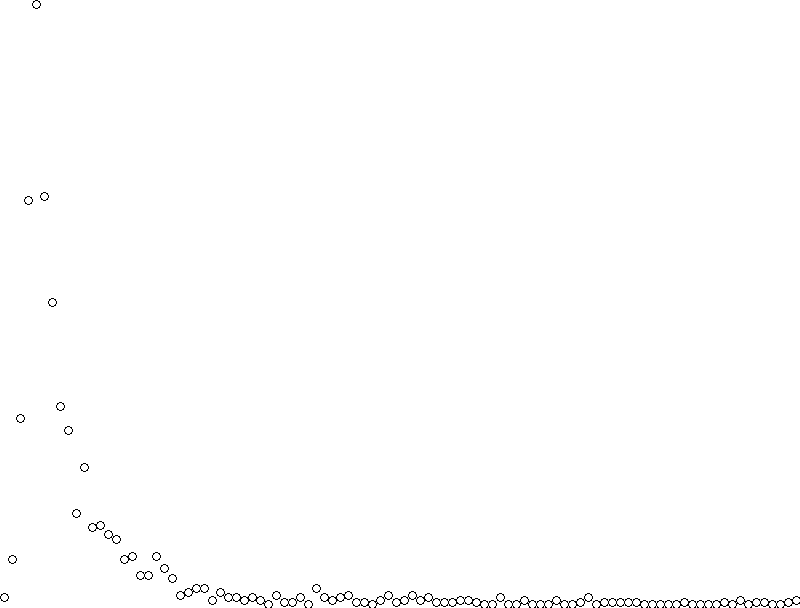
\includegraphics[width=0.95\linewidth]{figures/couto-vale/A02Ma032aa}}
                \caption{AA pauses \textbf{std ch}+\textbf{std ch}}
                \label{fig:gull}
        \end{subfigure}%
        \begin{subfigure}[b]{0.33\textwidth}
                \fbox{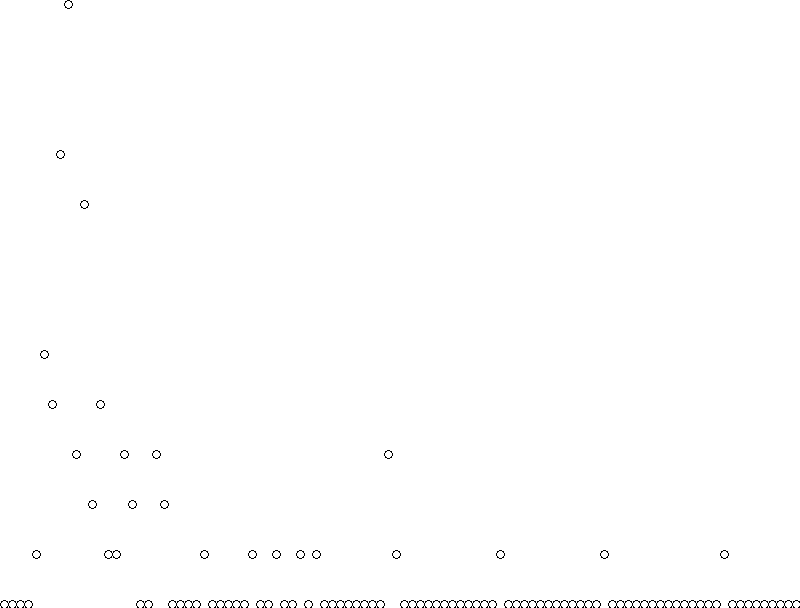
\includegraphics[width=0.95\linewidth]{figures/couto-vale/A02Ma032ba}}
                \caption{BA pauses \textbf{shift ch}+\textbf{std ch}}
                \label{fig:gull2}
        \end{subfigure}%
        \begin{subfigure}[b]{0.33\textwidth}
                \fbox{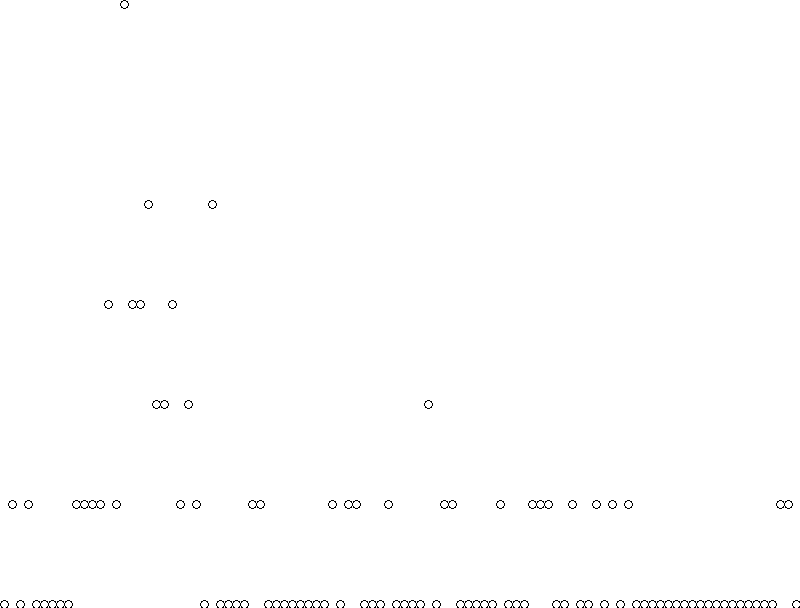
\includegraphics[width=0.95\linewidth]{figures/couto-vale/A02Ma032ab}}
                \caption{AB pauses \textbf{std ch}+\textbf{shift ch}}
                \label{fig:tiger}
        \end{subfigure}%
        \caption{Different writing pause lengths depending on AA, AB, BA pause type}
        \label{couto:fig:WritingPauses}
\end{figure}

\figref{couto:fig:WritingPauses} shows that AA \isi{pauses} were the smallest, BA \isi{pauses} (those containing a \textbf{shift key up} action) were longer, and AB \isi{pauses} (those containing a \textbf{shift key down} action) were the longest. In addition, it seems quite evident from the images that most \isi{pauses} lay between 0 milliseconds and about twice the size of the most frequent pause window. For this reason, I find twice the length of the maximum value of the most frequent window a good estimate of where the start of the \isi{typing pause} is. In the next section, I shall discuss how to classify typing \isi{pauses} according to their length in a meaningful way for the purpose of translation studies.

\largerpage[-1]
\subsection{Classes of typing pauses}
\label{couto:sec:ClassesOfTypingPauses}

Since we have an estimate of \isi{typing pause} that is seemingly imprecise, it is not very informative to look at very small \isi{pauses}. Therefore, what we count as typing \isi{pauses} close to zero are actually rough guesses that these might be typing \isi{pauses} and even rougher guesses that these might potentially be a motion pause. Any actual counting of such short \isi{pauses} would be very unreliable. We shall see in the following that they are nonetheless useful, even if imprecise.

Longer typing \isi{pauses} with large pause windows are likely to be less unreliable. For this reason, I found 128 milliseconds of estimated \isi{typing pause} length to be a good start. A \isi{typing pause} window starting at 128 milliseconds was called \emph{tpw\textsubscript{1}}. Since we need a way to compare similar-sized \isi{pauses} with each other in an order of magnitude way (not in very precise ways), I find a logarithmic scale for pause windows fitting for our task. Therefore, I conceived of pause windows with the time segment ${[}62\times 2^i, 62\times 2^{i+1}{[}$ where the minimum pause length is included and the maximum pause length is excluded. With this pause window formula, we would have the following \isi{typing pause} windows (tpw) in \tabref{couto:tab:7}.

\begin{table}%t7
\centering
\begin{tabular}{lrr}
\lsptoprule
Typing Pause Window & \multicolumn{1}{p{3cm}}{\mbox{Minimum Length} \mbox{(included)}} & \multicolumn{1}{p{3cm}}{\mbox{Maximum Length} \mbox{(excluded)}}\\
\midrule
tpw⁻ & 0 ms & 128 ms \\
tpw\textsubscript{1} & 128 ms & 256 ms \\
tpw\textsubscript{2} & 256 ms & 512 ms \\
tpw\textsubscript{3} & 512 ms & 1,024 ms \\
tpw\textsubscript{4} & 1,024 ms & 2,048 ms \\
tpw\textsubscript{5} & 2,048 ms & 4,096 ms \\
tpw\textsubscript{6} & 4,096 ms & 8,192 ms \\
tpw\textsubscript{7} & 8,192 ms & 16,384 ms \\
tpw\textsubscript{8} & 16,384 ms & 32,768 ms \\
tpw\textsubscript{$\infty$} & 32,768 ms & -- \\
\lspbottomrule
\end{tabular}
\caption{Typing pause windows}
\label{couto:tab:7}
\end{table}

The first and last lines of \tabref{couto:tab:7} indicate special \isi{typing pause} windows. Tpw\textsubscript{\={ }} are the pause windows where it is a mere guess that what we see is in fact a \isi{typing pause}, whereas tpw\textsubscript{$\infty$} indicate \isi{pauses} beyond 32 seconds. These \isi{pauses} are very infrequent and they occurred not more than 5 times per participant. Making cognitive claims on typing \isi{pauses} this long seemed rather unrealistic and I opted to discount them. \figref{couto:fig:TypingPausesPerWindow} shows the distribution of such \isi{pauses} for a particular \isi{translation process} from English to \ili{German} in our corpus.

\begin{figure}%f
  \centering
%   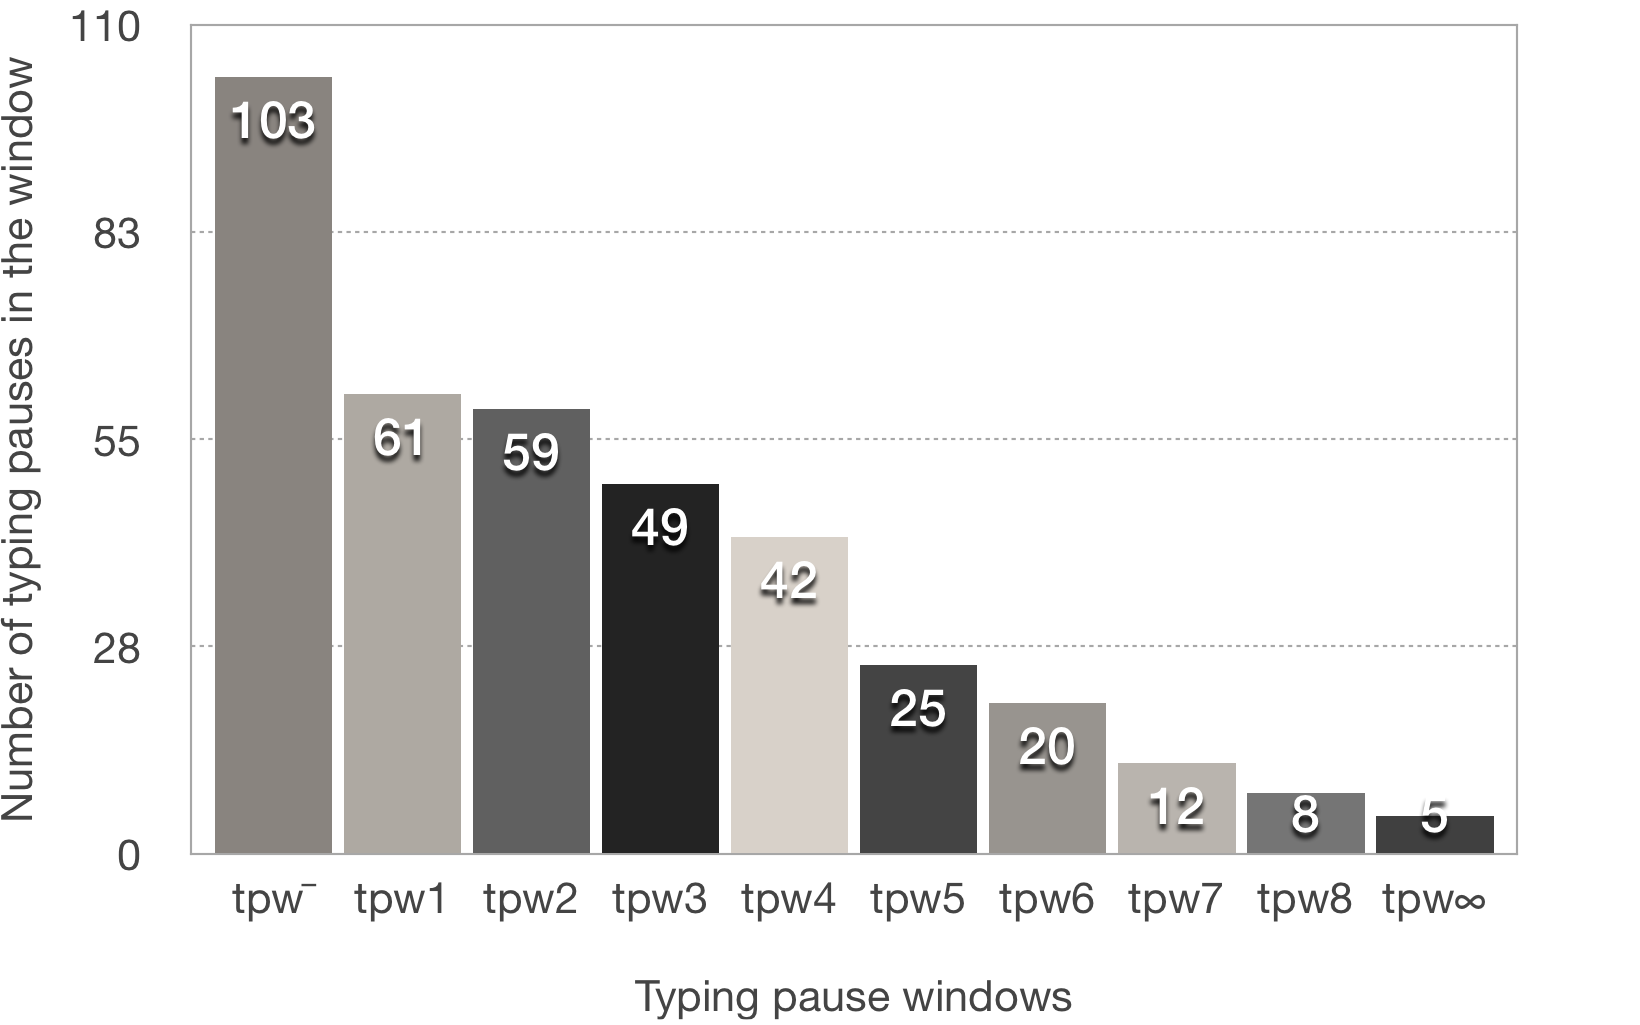
\includegraphics[width=0.75\linewidth]{figures/couto-vale/TPW1}
  \barplot{Typing pause windows}{Number of typing \isi{pauses} in the window}{tpw⁻,tpw1,tpw2,tpw3,tpw4,tpw5,tpw6,tpw7,tpw8,tpw∞}{
    (tpw⁻, 103)
    (tpw1, 61)
    (tpw2, 59)
    (tpw3, 49)
    (tpw4, 42)
    (tpw5, 25)
    (tpw6, 20)
    (tpw7, 12)
    (tpw8, 8)
    (tpw∞, 5)
  }  
  \caption{Frequency of typing pauses per window for a translation process}
  \label{couto:fig:TypingPausesPerWindow}
\end{figure}

The logarithmic windows of \figref{couto:fig:TypingPausesPerWindow} contain a decreasing number of typing \isi{pauses} as they get larger. The drop in \isi{typing pause} frequency between one window and the next is smooth, which is a good sign for a classification of this kind.

\subsection{Comparison with other approaches}
\label{couto:sec:ComparisonWithOtherApproaches}

Up to now in translation studies, two procedures to cut a \isi{translation process} into units have been tried, and both of them ignore the fact that the length of different writing \isi{pauses} (AA, BA, AB) correlate differently with \isi{typing pause} length. Both approaches considered gaps between two writing actions longer than a fixed threshold pause in translation, that is, these gaps were considered the boundaries of \isi{translation process} units. They were not understood as \isi{pauses} in writing nor as \isi{pauses} in typing nor as \isi{pauses} in finger motion.

The first fixed threshold used in translation studies was user-unspecific and was picked by the researcher him or herself. Early thresholds ranged between 5 and 6 seconds \citep{Hansen:1999wn,Hansen:2002wu,Alves:2003va,PACTE:2005vu}. The second approach to cut the writing process into units during translation was proposed by \citet{Dragsted:2004tj,Dragsted:2005vl}. Her approach consisted of finding a writing pause\footnote{Typing speed in her terms since she did not distinguish typing actions from writing actions} for each participant that `seemed to reveal a certain pattern of syntactic units\footnote{Here called \emph{grammatical structures}}'. The attempt is valid and it does reveal a certain patterning that looks similar to a word/group/phrase based cutting of the target \isi{text production}.

However, even though Dragsted's approach is much better at capturing the writing rhythm of fast and slow writers, it tells little about how much `cognitive' effort was put in each pause. It is also a poor indicator of \isi{cognitive effort} since it tends to find boundaries of \isi{translation process} units before all capital letters. This might lead researchers to believe that sentence beginnings and \ili{German} nouns are especially charged with \isi{cognitive effort}, when that is not really what is happening. It just takes longer for a person to type a capital letter than a small letter. Dragsted's approach also has the tendency to underestimate the \isi{cognitive effort} of writing \isi{pauses} between two small letters, which are typically shorter because less typing occurs during them. Examples \ref{couto:ex:17} and \ref{couto:ex:18} show respectively an undervaluation and and overvaluation of \isi{pauses}.

\begin{exe}%17
	\ex\label{couto:ex:17}
	\tt{$\cdot$\={ }A\u{ }s\u{ }p\u{ }e\u{ }k\u{ }t\u{ }$\cdot$} (TPW cut)\\
	\tt{$\cdot$•A\u{ }s\u{ }p\u{ }e\u{ }k\u{ }t\u{ }$\cdot$} (Dragsted's cut)
\end{exe}

\begin{exe}%18
	\ex\label{couto:ex:18}
	\tt{$\cdot$\u{ }z\u{ }u\u{ }$\cdot$57\={ }53$\cdot$2P\u{ }r\u{ }o\u{ }z\u{ }e\u{ }n\u{ }t\u{ }$\cdot$} (TPW cut)\\
	\tt{$\cdot$\u{ }z\u{ }u\u{ }$\cdot$•7\u{ }5\u{ }$\cdot$•P\u{ }r\u{ }o\u{ }z\u{ }e\u{ }n\u{ }t\u{ }$\cdot$} (Dragsted's cut)
\end{exe}

In Example \ref{couto:ex:17}, the tpw\textsubscript{\={ }} pause before the \textbf{`A' char insert} action was taken by Dragsted method as being significant whereas I estimate this pause to be on the borderline of being a \isi{typing pause} or not. It is barely longer than the regular gap between two typing actions of the translator. In contrast, Example \ref{couto:ex:18} shows an undervaluation of \isi{pauses}. Tpw\textsubscript{\={ }} and tpw\textsubscript{3} \isi{pauses} between \textbf{standard char insert} actions are not recognised, whereas a tpw\textsubscript{2} pause before a capital letter is. In other words, even though Dragsted's approach adapts better to the writing speed of each participant, it might give us a skewed view of \isi{pauses} in translation.

\section{Conclusion}
\label{couto:sec:Conclusion}

In the first part of this work, I went through a series of translation-unrelated linguistic phenomena that motivate \isi{pauses} during translation. The assumption that the boundaries of the grammatical structure under translation are the core and sole reason for there to be writing \isi{pauses} in the \isi{translation process} was put in check. Reasons for there to be \isi{pauses} vary between motion, typing, writing processes; in written products they vary between graphic, graphological, lexicogrammatical, and semantic strata, and in the lexicogrammatical stratum they vary between morpheme, word, group/phrase, and clause ranks. Each way of looking at the data allows us to identify different micro-units and corresponding macro-units of translation.

After listing some phenomena that occur in the \isi{translation process}, I revisited the issue of what is an adequate pause to take as indicator for \isi{cognitive effort}. As pointed out in the first part, the assumption that the length of a writing pause is a good indicator of \isi{cognitive effort} or translation-related activity does not hold. For this reason, I devised another indicator that results from estimating and classifying typing \isi{pauses}. This indicator seems less biased than the one used so far and it is modal, i.e. it is not a cut but a scalar value that increases together with the length of the pause at a logarithmic pace. 

Finally, for the future, given that we might have come to conclusions in prior publications based on skewed measurements, there is a large amount of work in need of reassessment. This work would include revisiting the claims that were defended with skewed measurements and which are now wide-spread assumptions in the field. We need to reassess whether these claims can still be sustained when analysing evidence in more detail and with less naïvité.

\section*{Acknowledgments}

The classification of \isi{typing pause} windows was performed at the \ili{German} Research Foundation (DFG) project TRICKLET (Translation Research in Corpora, Keystroke Logging and Eye Tracking), research grant no. NE1822/2-1. The linguistic annotation of hashtags was performed within the IfAAR -- English Linguistics.

%This space is reserved for an acknowledgement of the institution.%The acknowledgments should go immediately before the references.  Do not number the acknowledgments section. Do not include this section when submitting your paper for review.

\sloppy
\printbibliography[heading=subbibliography,notkeyword=this]
\end{document}

%%% Local variables:
%%% TeX-PDF-mode: t
%%% LaTeX-babel-hyphen: nil
%%% End:
